\documentclass[10pt,a4paper]{article}
\usepackage[utf8]{inputenc}
\usepackage{amsmath}
\usepackage{amsfonts}
\usepackage{amssymb}
\usepackage{graphicx}
\usepackage{float}
\usepackage[table, svgnames, dvipsnames]{xcolor}
\usepackage{makecell, cellspace, caption}
\usepackage{hyperref}

\author{Nicolò Brandizzi}
\title{Knowledge Representation Summary}
\date{November 2018}
\begin{document}


\begin{titlepage}
    \begin{center}
        \vspace*{1cm}
        
        \Huge
        \textbf{Knowledge Representation Summary}
        
        
        \vspace{1.5cm}
        
        Author:
        \textbf{Nicolò Brandizzi}\\
        \vspace{0.5cm}
        \Large
        Contributors:
        \textbf{}%add contributors here
        
        \vfill
        
        
\includegraphics[width=0.4\textwidth]{images/sapienza_logo.jpg}


        
        \vfill
        
  

        \vspace{0.8cm}
        
        
        \Large
        DIAG\\
        Sapienza\\
        November 2018

    \end{center}
\end{titlepage}


\tableofcontents
\newpage
\begin{abstract}
This is \textbf{free} material! You should not spend money on it.\\
This notes are about the \textit{Knowledge Representation} part taught by professor Daniele Nardi in the Artificial Intelligence class. Everyone is welcome to contribute to this notes in any relevant form, just ask for a pull request and be patient.\\ Remember to add your name under the contributors list in the title page when submitting some changes (if you feel like it).
\end{abstract}

\section{Logic based agents}
A \textbf{knowledge base} [KB] is a set of sentences in a knowledge representation language that express some assertion about the world.\\
We can either:
\begin{itemize}
\item \textit{Tell}: i.e. add new sentences to the KB or
\item \textit{Ask}: i.e. query what is known.
\end{itemize}
We can use both this actions to do \textbf{inference} in which we derive new sentences from old ones.\\

There are two ways of building a KB structure:
\begin{itemize}
\item \textbf{Declarative}: in which the agent is \textit{told} various aspects of the world \footnote{That is the designer add new sentences.} until it is capable of working in the environment.
\item \textbf{Procedural}: which encodes desired behavior directly in the program.
\end{itemize}

Finally an agent can be viewed at:
\begin{itemize}
\item \textit{Knowledge level}, where we specify what the agents knows and what are its goals. Or at
\item \textit{Implementation level}, where we need to specify the data structures used in the KB and the way to manipulate them.
\end{itemize}

\subsection{Logic}
Sentences must follow two principles in order to be considered \textit{correct}:
\begin{itemize}
\item \textbf{Syntax} holds when a sentence is \textit{well formed}, e.g. in mathematics "$x+y=4$" is correct while "$x3y +=$" is not.
\item \textbf{Semantic}  that defines the \textit{truth} of a sentence in respect to each possible world. For example the sentence $x+y=4$ is true in a world where $x=2,y=2$ but false when $x=1,y=4$.
\end{itemize}

Other than saying \textit{each possible world} when referring to the KB, we can use the word \textbf{interpretation}. Whereas possible worlds might be thought of as (potentially) real environments that the agent might or might not be in, interpretations are mathematical abstractions, each of which simply fixes the truth or falsehood of every relevant sentence.\\

Moreover a \textbf{model} $m$ is an interpretation of a sentence $\alpha$ if $\alpha$ is true in $m$ \footnote{Here the Russell-Norvig has a different concept of \textit{model} which is equal to the above \textit{interpretation (= each possible world = model)} . But Nardi prefer to make the distinction between the two so we will go with the Nardi flow (\textit{each possible world=interpretation $\neq$ model}).}. Given a set of the models of $\alpha$, $M(\alpha)$, we can derive the concept of \textit{entailment}:\\
A KB \textit{entails} a sentence $\alpha$ \footnote{That is the sentence $\alpha$ follows logically/is derived from KB.} if and only if, in every interpretation in which the KB is true \footnote{That is in every \textit{model} of the KB.}, $\alpha$ is also true:
\[KB \models \alpha \Leftrightarrow M(KB) \subseteq M(\alpha)\]
Note that $ M(KB) \subseteq M(\alpha)$ means that KB is a \textit{stronger assertion} than $\alpha$ since it \textit{rules out} more interpretation or possible worlds \footnote{There are less models in KB than in $\alpha$.}.

\paragraph{Example} Lets make an example to better understand this concepts.\\
We have the following sentences: 
\begin{itemize}
\item $\alpha=$ Overwatch is better than Fortnite.
\item $\beta=$ Everything is better than Diablo immortal \footnote{Don't you have phones?}.
\end{itemize}
Our KB is equal to $KB=\alpha \wedge \beta$, that is the KB knows that \textit{Overwatch is better than Fortnite \textbf{and} that Diablo immortal sucks}. We want to know:
\[KB \models \beta\]
i.e. we can derive from KB that Diablo immortal sucks.\\
We first need to check if $M(KB) \subseteq M(\beta)$, in other words if the KB has fewer true interpretation \footnote{Models.} than $\beta$. We know that the entailment holds since:
\begin{itemize}
\item The KB has two independent sentences, $\alpha,\beta$, correlated by an \textit{and} logic relationship, which result in fewer models.
\item  We are asking the KB for the truth of a sentence which is directly part of the KB itself; so that the set of models $M(KB)$ is a \textit{subset} of $M(\beta)$.
\end{itemize}

\paragraph{Model checking}  To know if $KB \models \beta$ we need to prove that $M(KB) \subseteq M(\beta)$. This can be done by \textbf{model checking}, that is enumerating all the possible interpretation where $KB$ is true and check if those are also models of $\beta$ \footnote{This is a direct implementation of the definition of entailment.}. For the above example we have:

\begin{table}[H]
\centering
    \begin{tabular}{|l|l|l|}
        \hline
        ~                              & KB    & \beta \\ \hline
        \alpha \wedge \beta            & \cellcolor{blue!25} True  & \cellcolor{blue!25} True  \\ 
        \neg \alpha \wedge \beta     & False & \cellcolor{blue!25} True  \\ 
        \alpha \wedge \neg \beta       & False & False \\ 
        \neg \alpha \wedge \neg \beta  & False & False \\
        \hline
    \end{tabular}
    \caption{Model checking for $KB\models\beta$}
\end{table}

\paragraph{Deduction} 
To better understand the difference between entailment and inference we should think of the \textit{set of all consequences} of KB as a haystack and $\beta$ as a needle. Entailment is like the needle being in the haystack; inference is like finding it.

Another way of computing the knowledge entailed by a KB is by a \textbf{deduction procedure}:
\[KB \vdash_i \beta\]
Which denotes that $\beta$ can be driven from KB by an \textbf{inference algorithm} $i$. 

\paragraph{Sound and Completeness} Given an inference algorithm $i$, if $i$ derives \textbf{only entailed} sentences from KB then it is considered \textbf{sound} \footnote{Or truth preserving.}, otherwise $i$ would make things up as it goes along (discovering of non-existing needles).\\
On the other hand \textbf{completeness} is also desirable: an inference algorithm is complete if it can derive any sentence that is entailed. For real haystacks, which are finite in extent, it seems obvious that a systematic examination can always decide whether the needle is in the haystack. For many knowledge bases, however, the haystack of consequences is infinite, and completeness becomes an important issue.

\paragraph{Difference between $\models$ and $\vdash$}
Having 
\begin{itemize}
\item $KB\models \alpha$
\item $KB \vdash \alpha$
\end{itemize}
The first symbol $\models$  is called \textbf{entailment} and means that $\alpha$ must be true in all of KB's models, that is KB  are true when $\alpha$'s interpretations are true \footnote{We can have some models of $\alpha$ which are not model in KB.}.\\
The other symbol $\vdash$ is read \textbf{derives} (KB derives $\alpha$) it can be joint with a sign denoting an inference rule, such as $KB \vdash_{MP}\alpha$ \footnote{Modus Ponens Section \ref{subsec:modusPonens}.} or $KB \vdash_{R}\alpha$ \footnote{Resolution Section \ref{sec:resolution}.} or both $KB \vdash_{R,MP}\alpha$. You can even ignore the set of inference rules and just write $KB \vdash\alpha$, in this case you are saying that \textit{it must exist a derivation \footnote{Obtained with some inference rule.} so that $\alpha$ is the last element of the chain}. You can verify the entailment with the derivation if and only if the inference rules you are applying are sound and complete.


\paragraph{Difference between \textit{deduction} and \textit{inference}}
Broadly speaking they are the same thing.\\
More specifically the \textit{deduction} is always referred to as a syntactic derivation, while \textit{inference} is a more generic  term which means that starting from KB we can conclude $\alpha$. So \textit{deduction} is tied to the $\vdash$ symbol, while \textit{infer} is more generic and can be used in both $\vdash, \models$

\newpage
\section{Propositional Logic}
Propositional logic is the simplest logic! \footnote{Not to understand...}

\paragraph{Syntax}
\label{par:syntax}
An \textbf{atomic sentence} is made of \textit{one} \textbf{propositional symbol} (for example $S$), which can be either \textit{True or False}.\\
\textit{True and False} are propositional symbols that are always True/False.\\
\textbf{Complex sentences} are propositional symbols joint together by the following \textbf{logical connective} (Figure \ref{fig:prop_synt}) :
\begin{itemize}
\item $\neg$ (not): $\neg S$ is the \textbf{negation} of $S$.
\item $\wedge$ (and): $S_1\wedge S_2$ is a \textbf{conjunction}.
\item $\vee$ (and): $S_1\vee S_2$ is a \textbf{disjunction}.
\item $\Rightarrow$ (implies): $S_1\Rightarrow S_2$ is an \textbf{implication}, where $S_1$ is the \textit{antecedent/premise} and $S_2$ is the \textit{consequent/conclusion}. Implication are known as \textbf{if-then} statement \footnote{If premise then conclusion.}.
\item $\Leftrightarrow$ (if and only if): $S_1\Leftrightarrow S_2$ is a \textbf{biconditional}.
\end{itemize}

\begin{figure}[H]
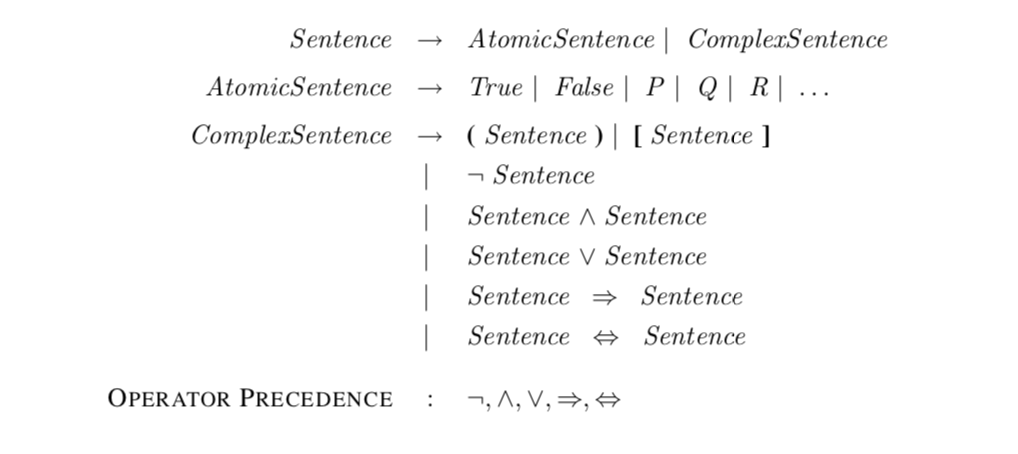
\includegraphics[scale=0.7]{images/prop_syntax.png}
\caption{Syntax summary for propositional logic}
\label{fig:prop_synt}
\end{figure}

\paragraph{Semantic}
The semantic defines the truth of a sentence in respect to a particular interpretation, that assign a truth value to every propositional symbol (Figure \ref{fig:truth_table}).

\begin{figure}[H]
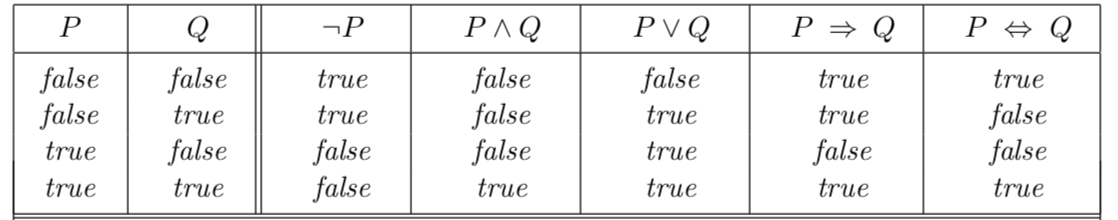
\includegraphics[scale=0.7]{images/truth_table.png}
\caption{Truth Table for propositional logic.}
\label{fig:truth_table}
\end{figure}

For  what regard the \textit{implies} symbol ($P \Rightarrow Q$) we need to specify that:
\begin{itemize}
\item It \textit{does not} need to have any causal/relevance link between the antecedent and the consequent. For example \textit{'5 id odd implies Tokyo is the capital of Japan'} is syntactically correct.
\item Any implication is true whenever the antecedent is false. This because we are saying \textit{'If P is true, then I am claiming that Q is true. Otherwise I am making no claim'}.
\item The only way for $P \Rightarrow Q$ to be false is if $P$ is true and $Q$ is false.
\end{itemize}


\paragraph{Inference}
Our goal is to prove that
\[KB \models \alpha\]
With the model checking approach we just need to enumerate all the possible interpretation and check that, when there is a model of KB then there is also a model of $\alpha$. This is done by assigning either \textit{true} or \textit{false} to every propositional symbol in any interpretation. But given $n$ symbols there are $2^n$ interpretations, thus the time complexity is $O(2^n)$, while the space complexity is $O(n)$ since we're using a depth-first approach. 

\subsection{Theorem Proving}
We can use a technique known as \textit{theorem proving} that consist in applying rules of inference directly to the sentences in our KB to construct a proof of the desired sentence without consulting models. If the number of models is large but the length of the proof is short, then theorem proving can be more efficient than model checking. We first need to introduce some concepts.

\paragraph{Logical equivalence} Two sentences $\alpha$ and $\beta$ are logically equivalent if they are true in the same set of interpretations, i.e. they have the \textbf{same set of models}. We write this as $\alpha \equiv \beta$. We can formalize this propriety by writing:
\[\alpha \equiv \beta \Longleftrightarrow \alpha \models \beta \wedge \beta \models \alpha\]
Following there are some standard logic equivalences (Figure \ref{fig:logic_equivalences}):


\begin{figure}[H]
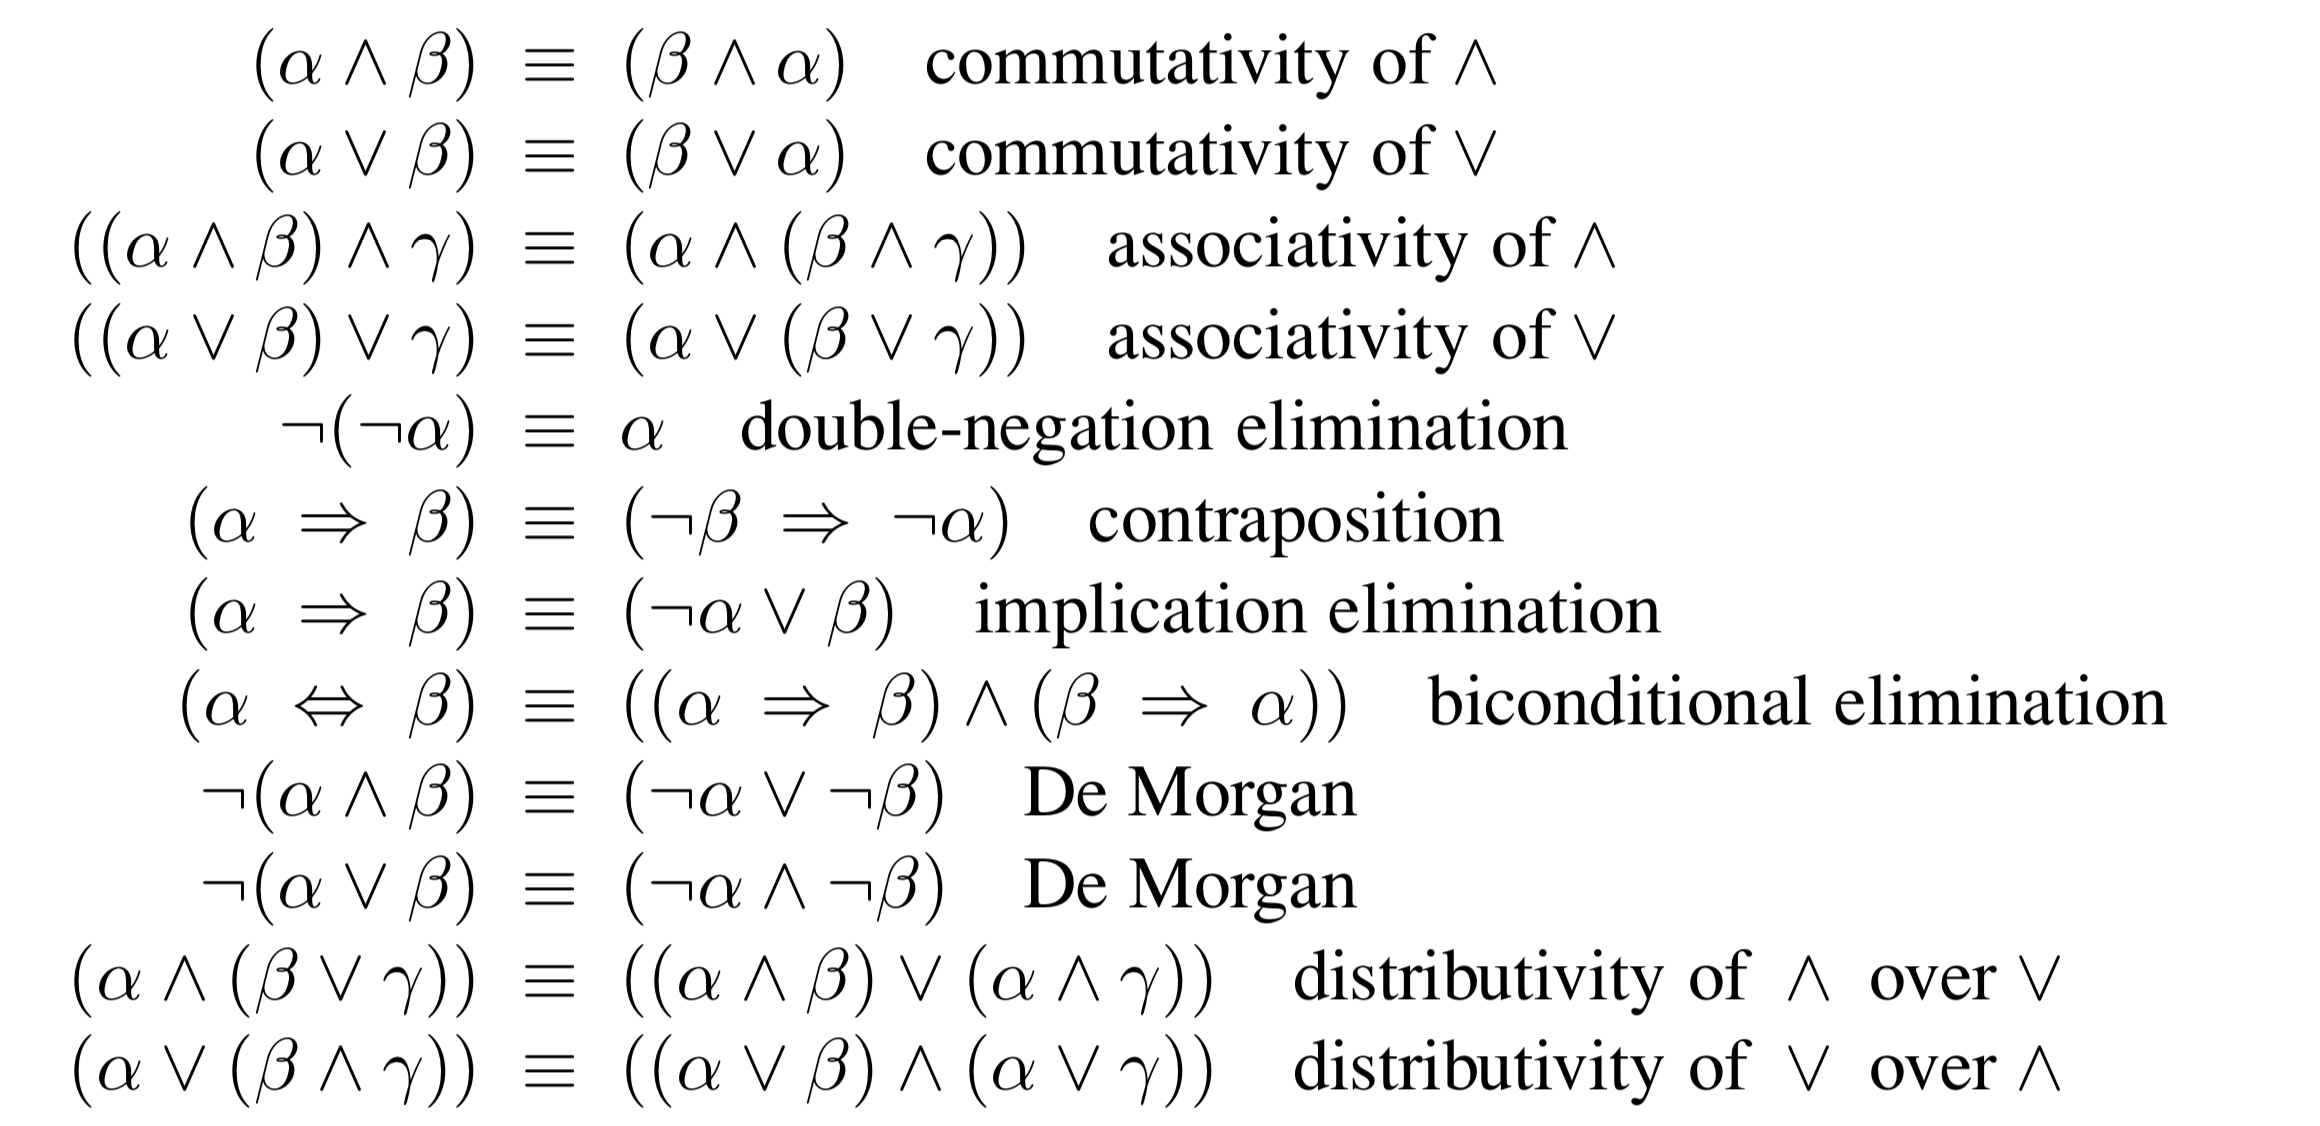
\includegraphics[scale=0.3]{images/equivalences.png}
\caption{Standard logic equivalences.}
\label{fig:logic_equivalences}
\end{figure}


\paragraph{Validity} A sentence is \textit{valid} if it is true in all interpretations \footnote{Also known as tautologies.}. For example: $A \vee \neg A$, $True$, $A \Rightarrow A$...\\
Validity can be tied to the deduction problem in the following way:\\
\textit{For every sentences $\alpha$ and $\beta$, $\alpha \models \beta$ if and only if the sentence $\alpha \Rightarrow \beta$ is valid}.

\paragraph{Satisfiability} A sentence is \textbf{satisfiable} \footnote{This problem is called SAT and it has been shown to be NP-complete.} if it is true in \textit{some} interpretation, i.e. it has some models. A sentence can be proved to be satisfiable by enumerating the possible implementations until a model is found \footnote{Model checking technique.}.\\
We can say that:
\begin{itemize}
\item \textit{$\alpha$ is valid iff $\neg \alpha$ is unsatisfiable}, or
\item \textit{$\alpha$ is satisfiable iff $\neg \alpha$ is not valid}.
\end{itemize}
Hence we can give another interpretation for entailment:
\[\alpha \models \beta \Longleftrightarrow (\alpha \wedge \neg \beta)\quad is \quad unsatisfiable\]
Which is also known as the \textbf{reductio ad absurdum} (proof by contradiction).

\subsubsection{Deduction in Propositional Logic}
\label{subsubsec:deduction}
We can use \textit{inference rules} to derive a proof \footnote{A proof is a chain of conclusion which leads to a desired goal.} of the interpretation truthfulness.
The idea behind finding a proof rather than using model checking is that the proof can ignore irrelevant proposition, no matter how many of them there are.\\
Usually this kind of rules are written in the form:
\[\frac{premisies}{conclusions}=\frac{A_1,A_2,...,A_n}{A}\]

Suppose we want to derive some formula \footnote{Or sentence.} $\alpha$ from the KB\footnote{Which is a set of formulas.} ($KB \vdash \alpha$), there must be a sequence of formulas $\alpha_1,...,\alpha_n$ such that:
\begin{itemize}
\item For every $i$ between $1...n$ either:
	\begin{itemize}
	\item $\alpha_i\in KB$, that is the formula $\alpha_i$ is in the KB. Or
	\item  $\alpha_i$ is a \textit{direct derivation} of $\alpha_{i-k},\ k\in [1,i-1]$ \footnote{$\alpha_i$  is a direct derivation of the previous formulas. In general $\alpha_i$ can depend on any subset of previous $\alpha$, it depends on the resolution rule used. }
	\end{itemize}
\item $\alpha=\alpha_n$, the chain of direct derivations brings to the formula we want to infer.
\end{itemize} 
Hence we can say that $\alpha_1,...,\alpha_n$ is a proof of $\alpha$ from the KB.
Finding a proof for a formula can implemented as a search where:
\begin{itemize}
\item \textit{Initial State}: is the KB  .
\item \textit{Operators}: are \textit{inference rules} (mentioned earlier).
\item \textit{Final state}: is the formula to be proven.

\end{itemize}



\paragraph{Basic proprieties}
We need to describe the proprieties of a inferring method $\mathcal{R}$ given a set of formulas $KB$ and a formula $A$. It is important to understand that by writing $\models A$ we are referring to the truthfulness of $A$ in all its interpretation, thus referring to the \textit{validity} of $A$.
\begin{itemize}
\item First we need to prove that an infer rule $\mathcal{R}$ is \textbf{sound}, to do so we need to prove that $A$ is \textbf{valid} given the fact that it can be derived with $\vdash_{\mathcal{R}}$.\\ 
First thing is to notice that there is no KB before the symbol since we want to prove $A$ being valid  regardless of the existence of any KB \footnote{That is a formula which is true in all models, for example $A \vee \neg A$.}.\\
But if we can derive $A$ with a deduction $\vdash$ then $A$ must be valid, so $\mathcal{R}$ is \textbf{sound} and we have: $KB \vdash_{\mathcal{R}} A$ implies $KB \models A$.
\item On the other hand, if $A$ is valid then it exist a derivation $\vdash_{\mathcal{R}} $ than let me derive it, so that $KB \models A$ implies $KB \vdash_{\mathcal{R}} A$, thus  $\mathcal{R}$ is \textbf{complete}.
\end{itemize}

\subsubsection{Inference and proof}
\label{subsec:modusPonens}

First thing first the truth tables we cited before are not associated with the inference rules. They are associated with the formulae! So you cannot apply any truth table to Modus Ponens, And Elimination and Resolution since it does not make sense.\\

Moreover atom and literal are the two basic elements for the construction of the formulae, in propositional logic $A$ is a propositional variable. But since we can have bot $A$ and $\neg A$ we say that $A$ is a literal which can be positive or negative.\\

The syntax (Section \ref{par:syntax}) allows you to build a formula regardless of the amount of free variable \footnote{This is use in general cases.}, when you have a formula with no free variables then its called a \textbf{sentence}. For example if we say:
\[A\wedge B \Rightarrow C\]
then its a formula, but if we associate a meaning to each literals:
\[Student \wedge SteamSales \Rightarrow Happy\]
Then it becomes a sentence.\\

On the other hand we used atom to indicate a formula for the estimations of predicates that has a predicates and some arguments. While in the propositional logic we have the propositional variable as a base element and an atom is a literal, in First Order Logic we have atoms.


\paragraph{Modus Ponens} We can ether use Modus Ponens:
\[\frac{\alpha \Rightarrow \beta,\quad \alpha}{\beta}\]
Which given $\alpha \Rightarrow \beta$ and $\alpha$ it can infer $\beta$. For example
\[\frac{man \Rightarrow mortal,\quad man}{mortal}\]
or
\[\Gamma =\lbrace feline \Rightarrow animal, cat \Rightarrow feline, cat \rbrace\]
Result in 
\[\Gamma \vdash_{MP} animal\]
Which mean that \textit{animal} can be derived from $\Gamma$ using the inference algorithm MP (Modus Ponens).\\

\paragraph{And Elimination}On the other hand we can use and elimination:
\[\frac{\alpha\wedge\beta}{\alpha}\]
more in general:
\[\frac{\alpha_1\wedge\alpha_2\wedge...\wedge \alpha_n}{\alpha_i}\]
Which works for any chain of conjunction and means that \textit{"if the rule $A=\lbrace\alpha_1\wedge\alpha_2\wedge...\wedge \alpha_n\rbrace$ is true, then for any $\alpha_i \in A$, $\alpha_i$ must be true as well"}, since we have an \textit{and} logical chain.\\

\paragraph{Monotonicity}
Finally \textbf{monotonicity} is the propriety of logical system  which says that the set of entailed sentences can only increase as information is added to the knowledge base:
\[if\ KB\models \alpha\ then \ KB\wedge\beta\models\alpha\]
Which means that inference rules can be applied whenever suitable premises are found in the KB; conclusion of the rule must follow regardless of what else is in the knowledge base \footnote{Nonmonotonic logics, which violate the monotonicity property, capture a common property of human reasoning: changing one's mind.}.

\paragraph{Inference rules}
We can use any of the equivalences from Figure \ref{fig:logic_equivalences} as inference rules, for example:
\[\frac{\alpha \Leftrightarrow \beta }{(\alpha \Rightarrow \beta)\wedge(\beta\Rightarrow\alpha)}\quad and\quad \frac{(\alpha \Rightarrow \beta)\wedge(\beta\Rightarrow\alpha)}{\alpha \Leftrightarrow \beta }\]

\subsection{Resolution}
\label{sec:resolution}
So far we did not provide any algorithm which can be considered \textbf{complete}, since the lack of some \textit{inference rules} may prevent the algorithm from reaching the goal. So we introduce the inference rule called \textbf{resolution} that yields a complete inference algorithm when coupled with any complete search algorithm (Section \ref{subsec:search_alg}).

\paragraph{Definitions}
Following there are some definitions:
\begin{itemize}
\item \textit{Formula}: is a set of literals joint by some logic connectives (e.g. a complex sentence).
\item \textit{Literals}: can be either one propositional symbol (or atom) or a negated atom. They are the same as an atomic formulae that is a formula that contains no logical connectives.
\item \textit{Clause}, is a \textit{disjunction} of literals, for example $L_1\vee L_2\vee...\vee L_n$
\item Moreover we introduce the $\bot$ and $\top$ symbols that are \textit{False} and \textit{True} respectively.

\end{itemize}





\subsubsection{Conjunctive Normal Form [CNF]}
\label{subsec:cnf}
\paragraph{Definition}
The key idea is that: \textit{every sentence of propositional logic is logically equivalent to a conjunction of clauses} ($Formula\equiv CNF(Formula)$) ; hence sentences expressed as a conjunction of clauses are said to be in CNF. You can either preserve equivalence when converting to CNF, but the number of clauses will be $2^n$, where $n$ is the number of literals; or you can preserve \textit{satisfiability} introducing new literals and linearly increase the size of the formula.\\



\paragraph{Example}
Let's make an example using:
\[A \Leftrightarrow (B \vee C)\]
In the following steps we make use of the formulae in Figure \ref{fig:logic_equivalences}

\begin{enumerate}
\item Use biconditional elimination and get: \\$(A \Rightarrow (B \vee C))\wedge((B \vee C)\Rightarrow A)$
\item Use implication elimination end get :\\$(\neg A \vee B \vee C)\wedge(\neg(B\vee C)\vee A)$
\item CFN requires the negation to be applied only to literals \footnote{When a sentence has negation symbols applied directly to literal then it is in \textbf{Negation normal form} [NNF]. For example $\neg(A\vee B)$ is not in NNF while $\neg A \wedge \neg B$ is.}, hence we need to use the De Morgan formula to move $\neg$ inwards: \\$(\neg A \vee B \vee C)\wedge((\neg B\wedge \neg C)\vee A)$
\item Finally we use the distributive law of $\vee$ over $\wedge$ and get:\\
$(\neg A \vee B \vee C)\wedge(\neg B \vee A)\wedge(\neg C \vee A)$
\end{enumerate}


\paragraph{Alpha-Beta Formulas}
There are some cases in which we need to separate dis/conjunction depending on the following formulas:
\begin{table}[H]
    \begin{tabular}{|l|l|l|l|}
        \hline
        C=\lbrace \alpha \rbrace     & C_1=\lbrace \alpha_1 \rbrace,C_2=\lbrace \alpha_2 \rbrace & C=\lbrace \beta \rbrace & C=\lbrace \beta_1, \beta_2\rbrace \\ \hline\hline
        \alpha =A \wedge B           & \alpha_1 = A,\ \alpha_2= B                                & \beta=A\vee B           & \beta_1= A ,\ \beta_2=B           \\ \hline
        \alpha =\neg(A\vee B)        & \alpha_1 =\neg A,\ \alpha_2= \neg B                       & \beta=A \Rightarrow B   & \beta_1=\neg A,\ \beta_2= B       \\ \hline
        \alpha =\neg(A\Rightarrow B) & \alpha_1=A,\ \alpha_2= \neg B                             & \beta=\neg(A\wedge B)   & \beta_1=\neg A,\ \beta_2= \neg B  \\
        \hline
    \end{tabular}
\caption{Alpha-Beta formulas for CNF}
\label{tab:alpha-beta}
\end{table}
As you can see from Table \ref{tab:alpha-beta} the alpha formulas result into two clauses \footnote{That is because there is a conjunction symbol. } $C_1,C_2$, while the beta formulas terminate in a single clause $C$ with two formulas \footnote{Note that I said formulas and not literals since both $\alpha_1,\alpha_2,\beta_1,\beta_2$ can be further simplified if they are not literals.}.

\paragraph{Algorithm}
Given a formula $F$ the algorithm for having the latter in CNF is the following:

\begin{enumerate}
\item Let $I=\lbrace F \rbrace$\footnote{The braces indicates that the $I$ is a set of clauses which will be joint by conjunctions.} be the initial state.
\item At the step $n+1$ we have that $I=\lbrace D_1,...,D_n \rbrace$ where $D_i$ is a disjunction containing some formulas $\lbrace A_1^i,...,A_k^i\rbrace$. 
\item If $A^i_j$ is not a literal then choose $D_i$ and do the following $\forall X_j \in D_i$:

	\begin{itemize}
	
	\item if $X_j$ is $\neg \top$ then replace it with $\bot$.
	\item if $X_j$ is $\neg \bot$ then replace it with $\top$.
	\item if $X_j$ is $\neg \neg X_j$ then replace it with $X_j$.
	\item if $X_j$ is $\beta$ formula then replace it with $\beta_1,\beta_2$.
	\item if $X_j$ is $alpha$ formula then replace $D_i$ with two clauses $D_i^1,D_i^2$ and add them to $I$. 

	\end{itemize}
	
\item Continue until every $D_i$ is made of literals.

\end{enumerate}


\paragraph{Expansion rules}
Finally note that the above rules can be written in the form of \textit{expansion rules} \footnote{Using the form introduced in Section \ref{subsubsec:deduction}.}:
\[\frac{\neg\neg A}{A}\quad \frac{\neg \top}{\bot}\quad \frac{\neg \bot}{\top}\quad \frac{\beta}{\beta_1,\beta_2}\quad \frac{\alpha}{\alpha_1 |\alpha_2}\]

\paragraph{Another Example}
Given the formula:
\[(P\Rightarrow (Q \Rightarrow(S\vee T)))\Rightarrow(T\Rightarrow Q)\]
We have that:
\begin{enumerate}
\item Use implication elimination (from now on it will be taken for granted) and get:
\[\neg(P\Rightarrow (Q \Rightarrow(S\vee T)))\vee(T\Rightarrow Q)\]
\item Use $\beta$ rule on disjunction:
\[C=\lbrace \beta_1= \neg(P\Rightarrow (Q \Rightarrow(S\vee T))),\beta_2=(T\Rightarrow Q)\rbrace\]
\item Use $\alpha$ rule on $\beta_1$ (negation of implication) and get:
\[C_1=\lbrace P,(T\Rightarrow Q)\rbrace,\quad C_2=\lbrace \neg  (Q \Rightarrow(S\vee T)),(T\Rightarrow Q)\rbrace \]
\item Use $\beta$ rule on $C_1$:
\[C_1=\lbrace P,\neg T, Q\rbrace,\quad C_2=\lbrace \neg  (Q \Rightarrow(S\vee T)),(T\Rightarrow Q)\rbrace \]
\item Use $\beta$ rule on $C_2$:
\[C_1=\lbrace P,\neg T, Q\rbrace,\quad C_2=\lbrace \neg  (Q \Rightarrow(S\vee T)),\neg T, Q\rbrace \]
\item Use $\alpha$ rule on $C_2$:
\[C_1=\lbrace P,\neg T, Q\rbrace,\quad C_2=\lbrace \neg  Q ,\neg T, Q\rbrace\quad C_3=\lbrace \neg(S \vee T),\neg T, Q\rbrace \]
\item Use $\alpha$ rule on $C_3$:
\[C_1=\lbrace P,\neg T, Q\rbrace,\quad C_2=\lbrace \neg  Q ,\neg T, Q\rbrace\quad C_3=\lbrace \neg S,\neg T, Q\rbrace\quad C_4=\lbrace \neg T,\neg T, Q\rbrace
\]
\end{enumerate}

\subsubsection{Horn clause}
\label{subsubsec:horn}

\paragraph{Definitions}
The definition for understanding Horn clauses are both reported in Figure \ref{fig:clauses} as well as in the following list:
\begin{itemize}
\item \textit{Definite clause}: is a disjunction of literals of which \textit{exactly one is positive}. For example:\[(\neg L_1 \vee \neg L_2 \vee L_3)\]
\item \textit{Goal clause}: is a disjunction of literals of which \textit{none is positive}. For example:\[(\neg L_4 \vee \neg L_5 \vee \neg L_6)\]
\item \textit{Horn clause}: is a disjunction of literals of which \textit{at most one is positive}. So you can either have \textit{definite clauses} or \textit{goal clauses}. For example:\[(\neg L_1 \vee \neg L_2 \vee L_3)\quad or\quad (\neg L_4 \vee \neg L_5 \vee \neg L_6)\]
\item \textit{Horn Form}: a KB is in Horn form if it is a conjunction of Horn clauses. For example:

	\begin{enumerate}
	\item $C \wedge (B\Rightarrow A)\wedge(C\wedge D\Rightarrow B)$
	\item $C \wedge (\neg B \vee A)\wedge(\neg(C\wedge D)\vee B)$
	\item $C \wedge (\neg B \vee A)\wedge(\neg C\vee \neg D \vee B)$
	\end{enumerate}
	
\end{itemize}

\paragraph{Motivation}
So why are we interested in definite/goal/Horne clauses?\\
\begin{itemize}
\item When we have a definite clause we can write it as an implication of conjunctions. For example:
\[(\neg L_1 \vee \neg L_2 \vee L_3)\quad becomes\quad (L_1 \wedge L_2)\Rightarrow L_3\]
In this case the premise is called the \textit{body} and the conclusion is called \textit{head}. Moreover a single positive literal is a \textit{fact} \footnote{Since a single literal can be viewed as a disjunction of one literal.}.
\item what is the advantage of having a goal clause??????????
\item Moreover inference in horn clauses can be done with the forward/backward chaining algorithm (Section \ref{subsec:chaining}).
\item Finally deciding entailment with Horn clauses can be done in time that is linear in the size of the knowledge base.




\end{itemize}

\begin{figure}[H]
\centering
\fbox{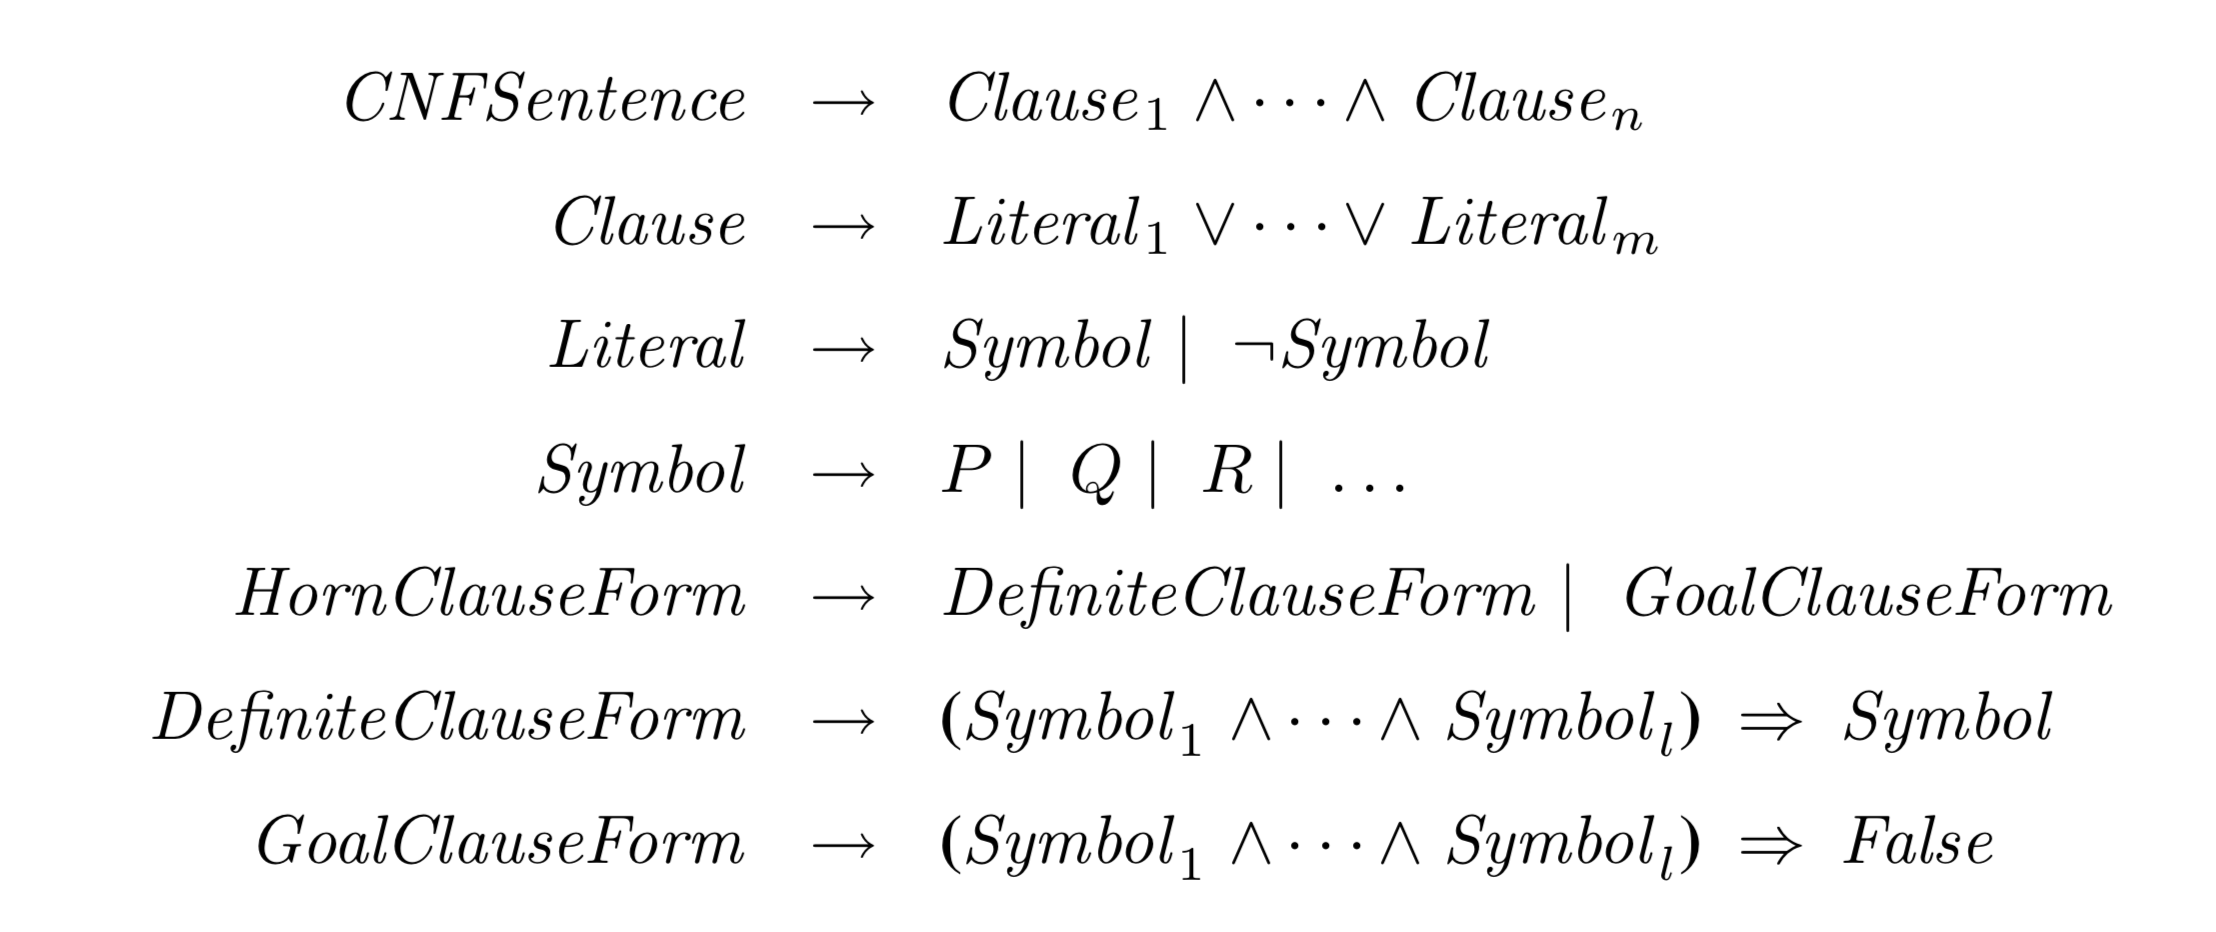
\includegraphics[scale=0.3]{images/horn_clause.png}}
\caption{Different types of clauses}
\label{fig:clauses}
\end{figure}

\subsubsection{Propositional Resolution }
\label{subsubsec:prop_resolution}
The key idea of the propositional resolution is that if I have two clauses $C_1,C_2$ \footnote{You should know by now that a clause is a disjunction of literals.} and one literal $L$ that appears with different sign in both $L \in C_1\ ,\neg L \in C_2$, then I can generate a new clause by joining $C_1 \vee C_2$ and removing $L,\neg L$ from them. That is because if I have a clause where a symbol appears with both sign, e.g. $C_3=L_1 \vee L_2 \vee \neg L_1$, then every interpretation I can give to $L_1$ will be indifferent since it will result in a model. 

\paragraph{English Example} Consider the following KB, with two clauses, trying to understand why can't I play Overwatch on Monday:
\begin{itemize}
\item $C_1$=\textit{"There is an exam the next day"} or \textit{"My pc is broken"} or \textit{"I'm tired"}
\item $C_2$=\textit{"There is no exam the next day"}
\end{itemize}
This is a special case of resolution called \textbf{unit resolution} in which I have a clause $C_1$ and a fact $C_2$. So, by examine the two clauses I can say that \textit{There is no exam the next day}, so the alternatives are either that \textit{my pc is broken} or that \textit{I'm tired}.\\
If we add another fact to the KB:
\begin{itemize}
\item $C_3$= \textit{I'm never tired on Mondays!}
\end{itemize}
Then the only logical conclusion why I can't play Overwatch on Monday is because \textit{my pc is broken.} \footnote{Sad me.}.

\paragraph{Formalization}
We can formalize the previous example for any given set of clauses:\\
Let there be two clauses:
\begin{align}
L=L_1\vee L_2 \vee...\vee L_n=\lbrace L_1,...,L_n\rbrace\\ 
P=P_1\vee P_2 \vee...\vee P_m=\lbrace P_1,...,P_m\rbrace
\end{align}
for any $n,m$.\\
Let there be a set of literals, $O=\lbrace O_1,...,O_k\rbrace$, which appears in both $L$ and $P$ but with opposite sign:
\[\forall O_i,\ O_i \in L, \neg O_i \in P\]
Se we can use resolution to join $P$ and $L$ \footnote{In this instance by joining we mean that we use the disjunction symbol between the two clauses.} and remove $O$ from the union:
\[\frac{L\quad P}{(L\cup P)\setminus O}\]
Which result will look like:
\[(L_1\vee L_2 \vee...\vee L_n\vee P_1\vee P_2 \vee...\vee P_m)\setminus (O_1\vee...\vee O_k)  \]

\paragraph{Formal Example}
Let's use the following KB:
\[KB=\lbrace C_1=\lbrace\neg P,Q,\neg P\rbrace,\quad C_2=\lbrace P,\neg L\rbrace \rbrace\]
We first apply \textbf{factoring} to remove the double $\neg P$ in $C_1$, thus having:
\[KB=\lbrace C_1=\lbrace\neg P,Q\rbrace,\quad C_2=\lbrace P,\neg L\rbrace \rbrace\]

Given a formula $\alpha=\lbrace Q,\neg L\rbrace$ we want to know if $KB \models \alpha$, that is $(KB \vee \neg \alpha)$ is unsatisfiable, that is  $(KB \vee \neg \alpha) \vdash_{\mathcal{R}} \{\}$ \footnote{Note that $\{\}$ is the empty clause which is equivalent to \textit{False}.}. We have that:
\[(KB \vee \neg \alpha)=\lbrace C_1=\lbrace\neg P,Q\rbrace,\quad C_2=\lbrace P,\neg L\rbrace,\quad C_3=\lbrace \neg Q \rbrace,\quad C_4=\lbrace \neg \neg L=L\rbrace \rbrace\]
The procedure works as follow:
\begin{enumerate}
\item Resolve $C_1$ with $C_2$ which outputs:
\[C_5=\frac{\lbrace\neg P,Q\rbrace\quad \lbrace P,\neg L\rbrace}{\lbrace\neg L,Q\rbrace}=\lbrace\neg L,Q\rbrace\]
So that we have:
\[ C_3=\lbrace \neg Q \rbrace,\quad C_4=\lbrace L\rbrace ,\quad C_5=\lbrace\neg L,Q\rbrace \]
\item Resolve $C3$ and $C_5$ in the same way and get:
\[C_4=\lbrace L\rbrace ,\quad C_6=\lbrace\neg L\rbrace \]
\item Finally resolve $C_4$ and $C_6$ and get the empty clause $\{\}$
\end{enumerate}

We just demonstrated that $(KB \vee \neg \alpha) \vdash_{\mathcal{R}} \{\}$ thus that $KB\models \alpha$. Notice that these passages can be written in a tree form as shown in Figure \ref{fig:res_expansion}.
\begin{figure}[H]
\centering
\fbox{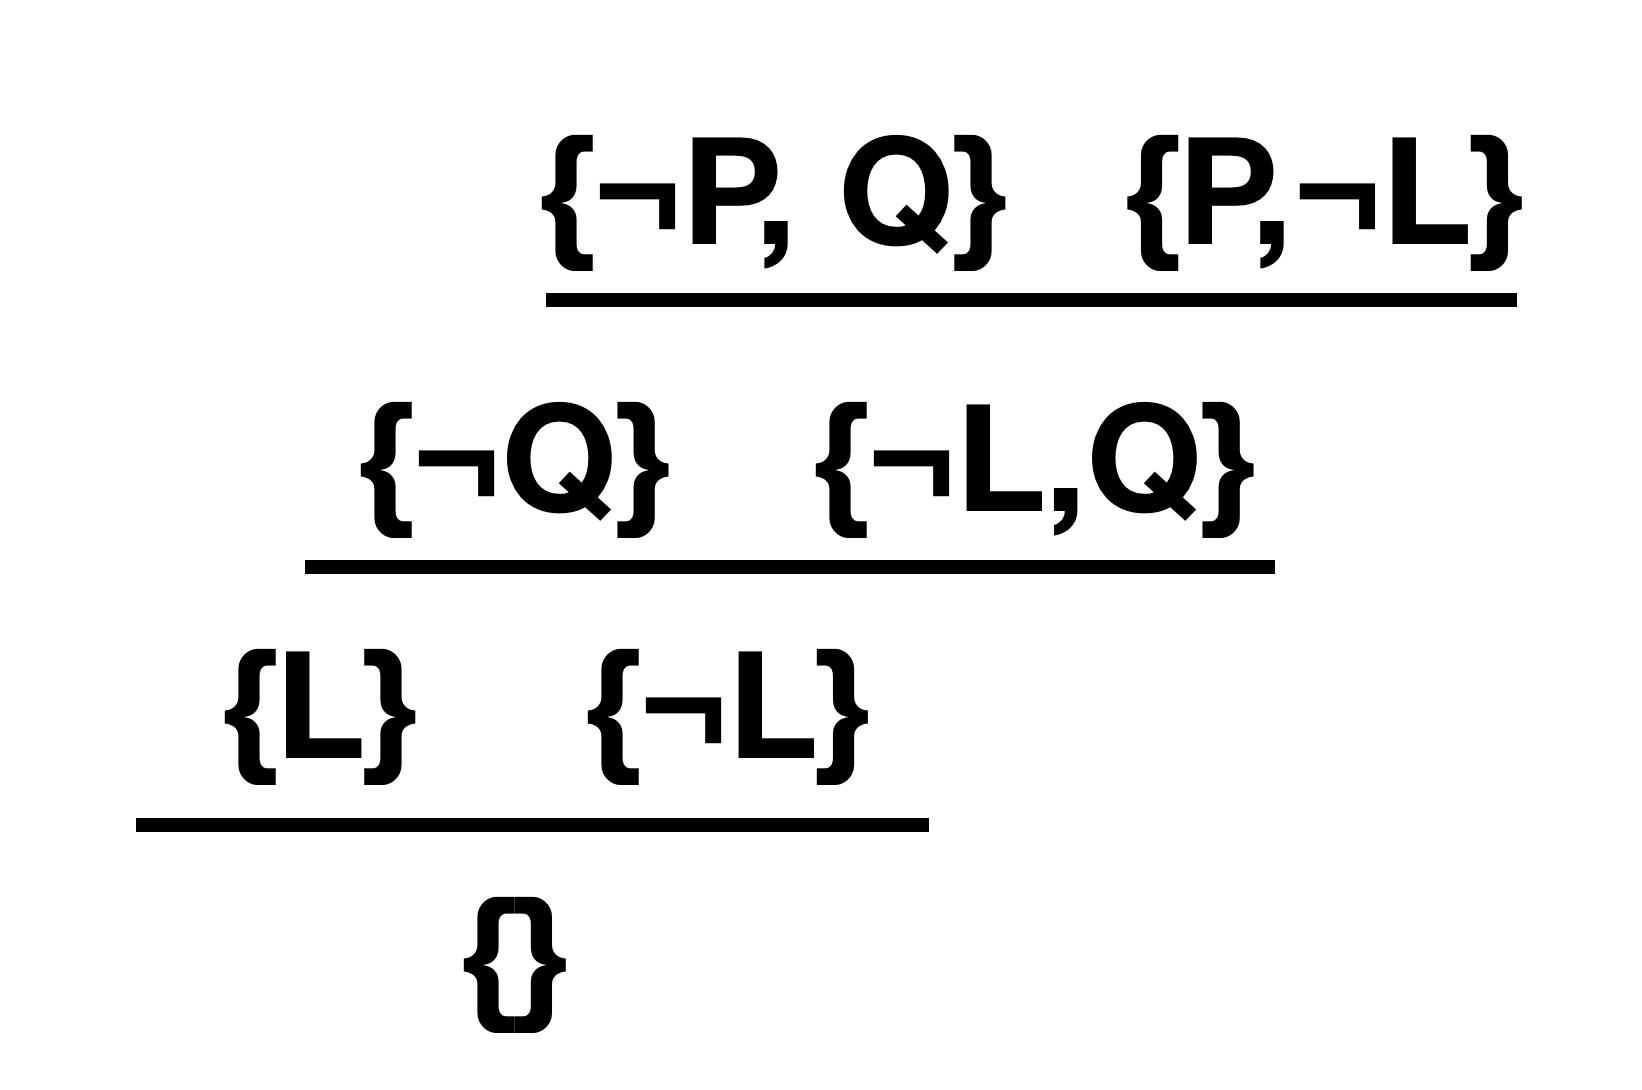
\includegraphics[scale=0.3]{images/res_expansion.png}}
\caption{Resolution steps shown in tree form}
\label{fig:res_expansion}
\end{figure}

\paragraph{Satisfiability of Resolution} We start by having two clauses $C_1=\lbrace L_1,...,L_n\rbrace$, $C_2=\lbrace P_1,...,P_m\rbrace$ and a literal that is the same in each clause but with a different sign $L_i=\neg P_j=K$, i.e. if $L_i$ is \textit{True} then $P_j$ is \textit{False}. We want to prove that $\lbrace C_1 \cup C_2 \rbrace \setminus \{K\}$ is satisfiable.\\
Suppose $C_1$ and $C_2$ are satisfiable, i.e. there exists a model $\mathcal{M}$; such that $\mathcal{M}\models C_1$ and $\mathcal{M}\models C_2$, and that $L_i$ is true in $\mathcal{M}$; it follows that $\neg L_1$ is \textit{False} in $\mathcal{M}$, thus $P_j$ is \textit{True} in $C_2$ and therefore $C_2$ must be \textit{True} in $\mathcal{M}$. Consequently, $C_1\cup C_2$ is true in $\mathcal{M}$. Since $\mathcal{M}$ is a model of $C_1,C_2$ by hypothesis, $C_1\cup C_2$  is true in M.\\
Same goes with $\mathcal{M}\models \neg L_i$.


\paragraph{Completeness of resolution} We introduce the notion of \textbf{resolution closure} $RC(S)$ of a set of clauses $S$ that  is the set of all clauses derivable by repeated application of the resolution rule to clauses in $S$ or their derivatives.\\
It is easy to understand that $RC(S)$ is finite because there are only finitely many distinct clauses that can be constructed out of the symbols $P_1, . . . , P_k$ that appear in $S$ \footnote{This is true only if we are using the factoring step to remove duplicate literals.}.\\ 

Now let us consider the \textbf{ground resolution theorem} which states:
\textit{If a set of clauses is unsatisfiable, then the resolution closure of those clauses contains the empty clause}; that is :
\[S\quad unsatisfiable\quad iff\quad \{\}\in RC(S)\]
Now let's prove this the other way around, we want to prove that:
\[S\quad satisfiable\quad iff\quad \{\}\notin RC(S)\]
First we build a model of $RC(S)$ with the following procedure.\\ For $i$ in $range(k)$:
\begin{itemize}
\item Given a clause $C_k \in S$ that contains $\neg P_i \in C$ and all its other literals are set to \textit{False}, $C_k=false\vee...\vee false\vee \neg P_i$; assign $False$ to $P_i$, so to make $C_k$ true.
\item Otherwise assign \textit{True} to $P_i$.
\end{itemize}
So now we have a model of $S$. Since we must prove that $RC(S)$ is satisfiable, thus have some models, let's assume that what we just got is not a model, then we must have been wrong at some iteration $i$. That is setting the symbol $P_i$ causes some clause $C$ to becomes false, since we \textit{do not have a model} all the other clauses must be already false. So $C$ can be one of the following possibilities:
\begin{itemize}
\item $C=false\vee...\vee false\vee P_i$
\item $C=false\vee...\vee false\vee \neg P_i$
\end{itemize}
If \textit{only one} of the two is in $RC(S)$ then the algorithm would assign the right value to make $C$ true. So the only way to have $C$ false is that \textit{both} possibilities are in $RC(S)$, but this is impossible since $RC(S)$ is \textbf{closed under resolution}, that is the two possibilities would have been resolved by the algorithm.

\subsection{Chaining}
\label{subsec:chaining}


\subsubsection{Forward Chaining}

\paragraph{Definition}
Determines if a single proposition symbol $q$ \footnote{What is asked to the KB, i.e. the query.} is entailed by a KB of definite clauses \footnote{Definite clauses means the KB contains either facts (positive literals) or implication with an \textit{atomic} conclusion and, for premise, either an atom or a conjunction of literals. }. It begins from known facts in the knowledge base \footnote{For this reason it is called \textbf{data driven}.}. If all the premises of an implication are known, then its conclusion is added to the set of known facts. This process continues until the query $q$ is reached or until no further inferences can be made. The main point to remember is that it runs in linear time.

\paragraph{Example}
Given the following KB:
\begin{itemize}
\item $P \Rightarrow Q$, equal to $\neg P \vee Q$ (definite clause)
\item $L \wedge M \Rightarrow P$, equal to $\neg L \vee \neg M \vee P$ (definite clause)
\item $B \wedge L \Rightarrow M$, equal to $\neg B \vee \neg L \vee M$ (definite clause)
\item $A \wedge P \Rightarrow L$, equal to $\neg A \vee \neg P \vee L$ (definite clause)
\item $A \wedge B \Rightarrow L$, equal to $\neg A \vee \neg B \vee L$ (definite clause)
\item $A$, (known fact, since positive literal)
\item $B$, (known fact, since positive literal)
\end{itemize}
We query Q \footnote{That is we ask the KB about the truthfulness of Q.}.\\
 The KB can bee seen as an \textbf{AND-OR Graph} where the implications are $or$ arches while the $\wedge$ are $and$ arches (Figure \ref{fig:forward_graph_1}).\\


\begin{figure}[t]
\centering
\fbox{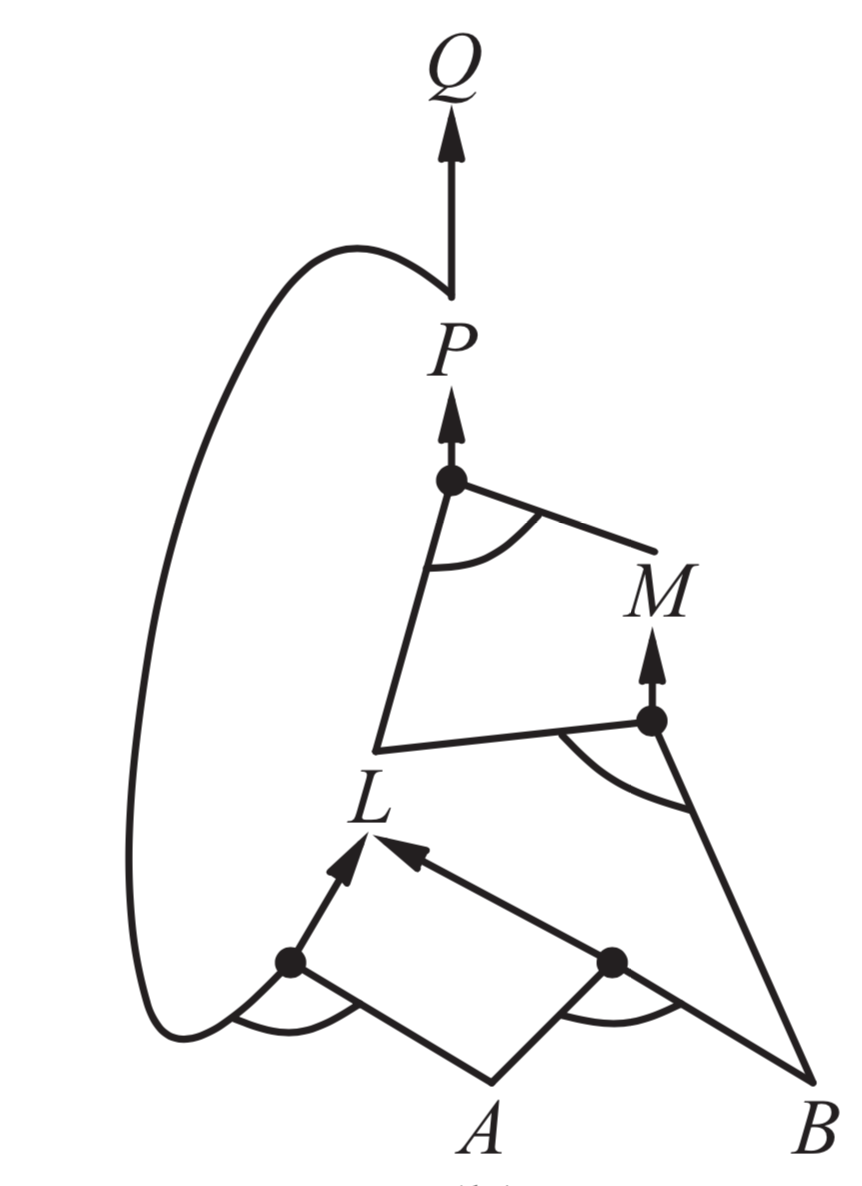
\includegraphics[scale=0.3]{images/forward_graph.png}}
\caption{AND-OR graph for definite clause KB}
\label{fig:forward_graph_1}
\end{figure}
The flow of the algorithm works as illustrated in Figure \ref{fig:forward_graph_2}.


\begin{figure}[H]
\centering
\fbox{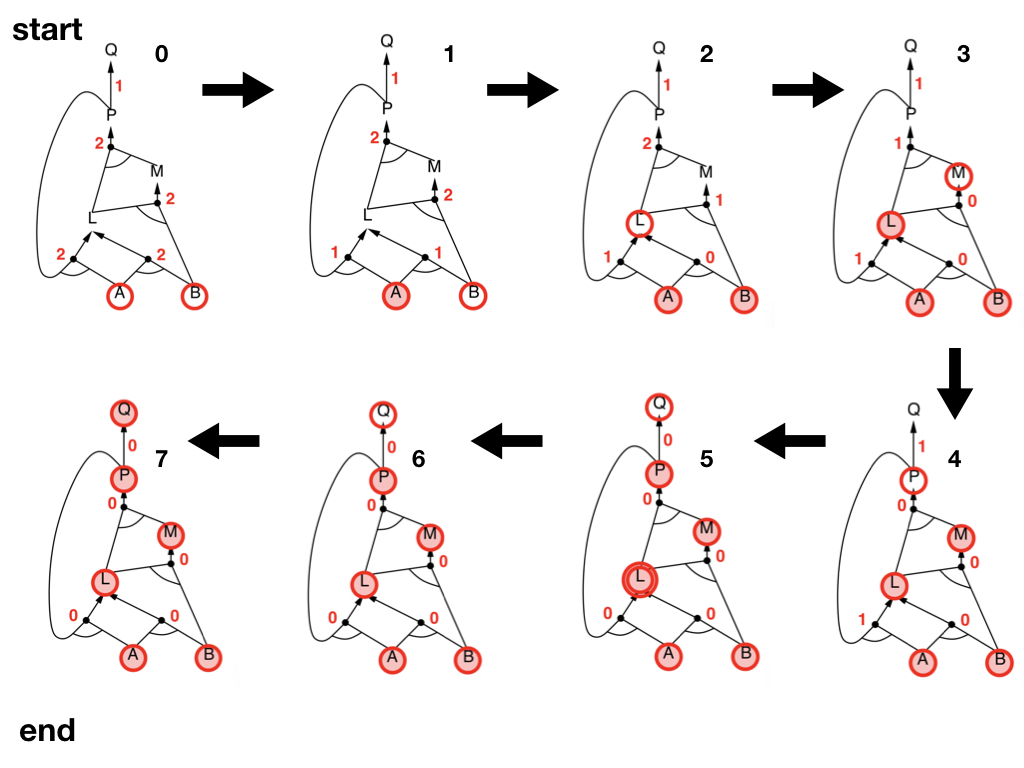
\includegraphics[scale=0.3]{images/forward_graph_2.jpeg}}
\caption{Forward Chaining for KB graph}
\label{fig:forward_graph_2}
\end{figure}


\paragraph{Proof}
We can affirm that the algorithm is \textbf{sound} since every step is an application of Modus Ponens.\\
For the \textbf{completeness} we need to prove that every possible atomic sentence can be derived from the KB. We first introduce the notion of \textbf{fixed point} which is a state of the algorithm in which no more inference can be done; then we consider to be in the final state $m$ that is a model \footnote{In which there has been various assignment of \textit{True/False} for the literals.} because we cannot apply Modus Ponens to any other clause.\\
Since the final state is in Horn form \footnote{As the whole KB.} we have a conjunction of disjunctions, so to be a model \footnote{True interpretation.} every clause must be \textit{True}. To prove this let's consider the opposite:
\begin{itemize}
\item Let's take a generic clause $C=a_1\wedge...\wedge a_n\Rightarrow b$ in $m$. This clause have a general number of conjunctions $n$ in its premise.
\item Suppose that $C$ is false in $m$.
\item For an implication to be \textit{False} we need the premise $a_1\wedge...\wedge a_n$ to be \textit{True} and the conclusion $b$ to be \textit{False}.
\item But if that is the case I would apply Modus Ponens again $\frac{a_1\wedge...\wedge a_n\Rightarrow b\quad a_1\wedge...\wedge a_n}{b}$ and conclude $b$ True, so in fact I'm not in a fixed point and this contradicts the assumption.
\end{itemize}


We can conclude, therefore, that the set of atomic sentences inferred at the fixed point defines a model of the original KB. Furthermore, any atomic sentence q that is entailed by the KB must be true in all its models and in this model in particular. Hence, every entailed atomic sentence q must be inferred by the algorithm.

\subsubsection{Backward Chaining}
On the other hand the backward chaining works its way from the query $q$ \footnote{Note that if the query is true the algorithm stops immediately.} and find those implication which conclusions are equal to $q$. If all the premises of a given implication which resolve in $q$ are true then we can conclude that $q$ is true itself.\\
This kind of reasoning is called \textbf{goal directed} reasoning and it usually works in linear size in respect to the size of the KB.



\subsection{Proposal for model checking}
\label{subsec:search_alg}
In this section, we describe two families of efficient algorithms for general propositional inference based on model checking: One approach based on backtracking search, and one on local hill-climbing search. Notice that these algorithms are used for checking the \textbf{satisfiability} (SAT) of a problem

\subsubsection{DPPL}
Also known as David-Putnam, Logemann, Loveland algorithm, it takes as input a sentence in conjunctive normal form (Section \ref{subsec:cnf}) and uses a recursive depth-first enumeration of all possible interpretations. To speed up the algorithm we can introduce some improvements.

\paragraph{Early Termination} A clause is true if \textit{any} literal is true \footnote{Remember that a clause is a disjunction of literals of the form $C_1\vee C_2\vee...\vee C_n$.}, hence if we encounter a true literal in a clause we can stop looking at it and give it the value \textit{true} \footnote{Similarly a sentence (conjunction of clauses) is false if \textit{any} clause is false.}.\\
For example having $(A\vee B)\wedge(A \vee C)$, if $A$ is true then we do not need to look for the values of $B,C$.

\paragraph{Pure Symbol} is a symbol which always appears with the same "sign", i.e. negated or not, so it can be assigned a value once for all the clauses.
For example:
\[(A\vee\neg B)\wedge (\neg B \vee \neg C)\wedge(C \vee A)\]
In this case the literal A is a pure positive symbol, B is a pure negative while C is impure.

\paragraph{Unit clause} is a clause with only one literal. This can be either because
\begin{itemize}
\item We have a clause with just one literal (fact). Or
\item We have a clause with multiple literals that are false \footnote{Since clauses are disjunction, false literals can be removed if there are some other that can assume the value true.} except for this last one \footnote{This is also called \textbf{unit propagation}.}.
\end{itemize}

\paragraph{Component analysis} We can divide clauses into independent subset when they \textit{do not share} any common literal. By dividing them we can parallelize the job as well as prune large part of the state space 	\footnote{No necessity to check the constraint of a literal in other clauses which do not have it. }

\paragraph{Variable and Value ordering} A general rule is to always try the value \textit{true} before \textit{false}. While the \textbf{degree heuristic} suggests choosing the variable that appears most frequently over all remaining clauses \footnote{Everything we saw in the planning part of the course.}.

\paragraph{Intelligent Backtracking} Also discussed in the Planning part of the course, intelligent backtracking keeps tracks of conflicts \footnote{Literals that may create a conflict with other literals.} so to cut off useless searches steps.

\paragraph{Random restarts} When the algorithm gets stuck for a long time execute a restart from the root point.

\paragraph{Clever indexing} at implementation level.

\subsubsection{Local Search Algorithm}
These algorithms works by flipping the truth value of one symbol at a time. The search space usually contains many local minima, to escape from which various forms of randomness are required. 

\paragraph{GSAT} Missing

\paragraph{WALKSAT} 
The algorithm picks an unsatisfied clause and picks a symbol in the clause to flip. It chooses randomly between two ways to pick which symbol to flip: 
\begin{itemize}
\item A \textit{min-conflicts} step that minimizes the number of unsatisfied clauses in the new state.
\item A \textit{random walk} step that picks the symbol randomly.
\end{itemize}
This type of algorithm is very similar to simulate annealing studied in the Local search part.
WALKSAT may end with the following outcomes:
\begin{itemize}
\item A model; thus the input sentence is satisfiable.
\item A failure; then there are two possibilities:

	\begin{itemize}
	\item Either the sentence is unsatisfiable, or
	\item The algorithm needs more time to complete the search \footnote{Note that if there is no limit to the number of flips and the sentence is unsatisfiable then the algorithm may never end.}.
	\end{itemize}
\end{itemize}

\subsubsection{Random SAT problem}
Depending on the number of clauses $m$ and symbols $n$ we can either have an \textit{under-constraint} problem ($n>m$) or a \textit{over-constraint} problem ($m>n$) \footnote{Giving that each symbol may not appear twice in a clause and no clauses may appear twice in the sentence.}. Given the ration $r=m/n$, when the ratio approaches zero then the probability of the problem to be satisfiable approaches one and vice versa. As you can see from Figure \ref{fig:sat} around the value $r=m/n=4.3$ the probability for the sentence to be satisfiable approaches zero.


\begin{figure}[H]
\centering
\fbox{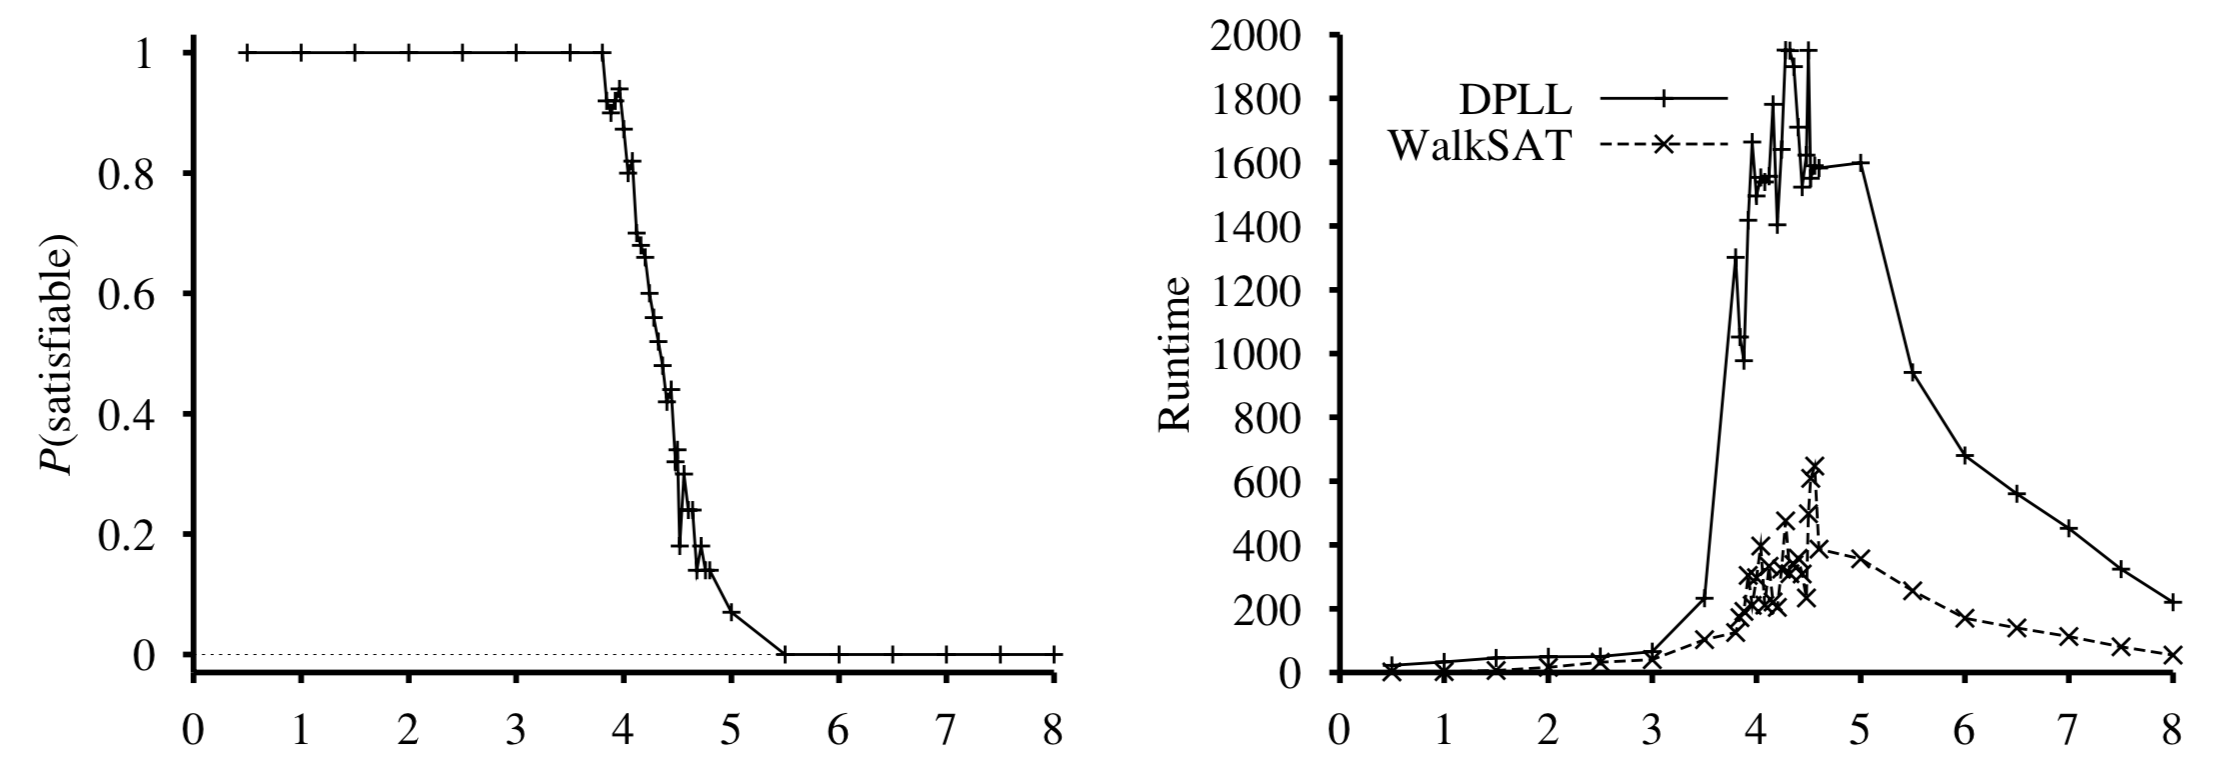
\includegraphics[scale=0.3]{images/sat.png}}
\caption{(Left) Graph showing the probability that a random  sentence with n = 50 symbols is satisfiable, as a function ratio m/n. (Right) Graph of the median run time on random sentences. The most difficult problems have a ratio of about 4.3.}
\label{fig:sat}
\end{figure}

\newpage
\section{First Order logic}
Having $A\Rightarrow B \Rightarrow C$ is read as $A\Rightarrow (B \Rightarrow C)$ not $(A\Rightarrow B) \Rightarrow C$

If we can use   modus ponens then we can use resolution, but if we can use resolution  we can't use modus ponent, since generalize modus ponens can be only for definite horn clauses.



\end{document}
